% 07 - PLC VISUALIZATION V1
% ==============================================================
\sectionintro{07 · Supervision}{PLC Visualization V1}{Une vue intégrée à TwinCAT XAE expose l'état du cycle et fournit les commandes nécessaires à la simulation.}

\begin{figure}[h]
  \centering
  \fcolorbox{ekline}{white}{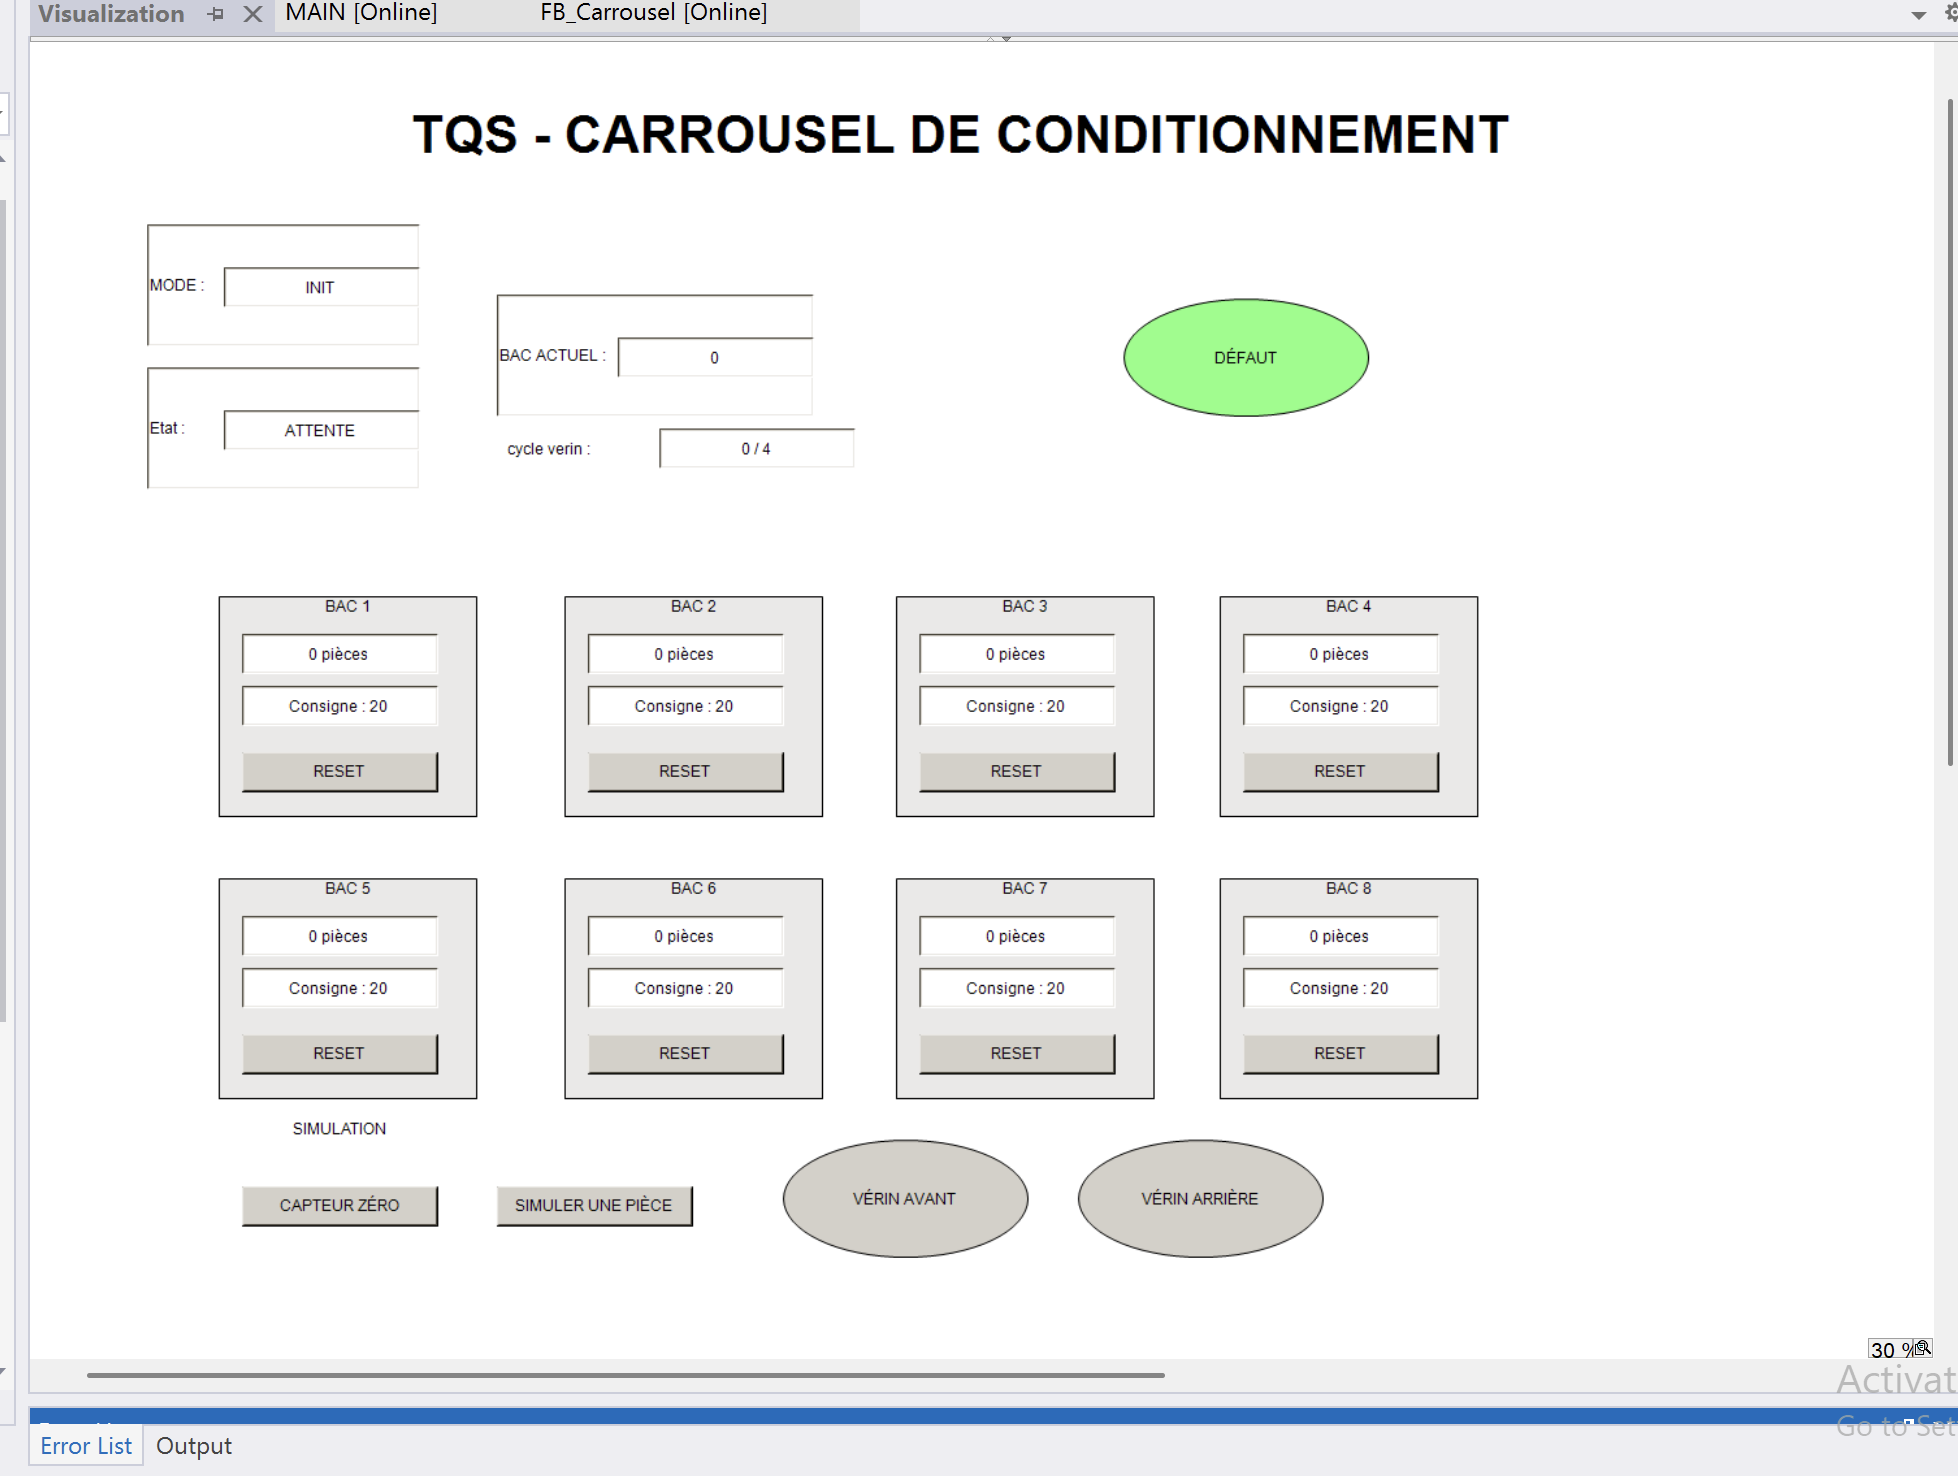
\includegraphics[width=.82\linewidth]{../images/VISU1.png}}
  \caption{PLC Visualization V1 en ligne dans TwinCAT XAE ; les valeurs correspondent à l'instant de la capture.}
\end{figure}

\vspace{-2mm}
\twocolpage{
  \subsection{Objets du projet}
  \begin{primarycard}
    \small
    \texttt{Visualization Manager.TcVMO} déclare \texttt{Visualization} comme vue de démarrage. \texttt{Visualization.TcVIS} contient les éléments et leurs liaisons ; \texttt{GlobalTextList.TcGTLO} porte les libellés et formats. Ces trois objets sont inclus dans \texttt{PLC\_Carrousel.plcproj} avec les bibliothèques de visualisation requises.
  \end{primarycard}

  \begin{notebox}{Nature de l'interface}
    Il s'agit de la PLC Visualization intégrée au projet automate. Ce n'est pas une application TwinCAT HMI V2.
  \end{notebox}
}{
  \subsection{Informations et commandes liées à \texttt{MAIN}}
  \begin{tabularx}{\linewidth}{@{}L{33mm}Y@{}}
    \toprule
    \textbf{Zone} & \textbf{Variables réellement utilisées}\\
    \midrule
    État global & \texttt{sModeVisu}, \texttt{sEtatCycleVisu}, \texttt{nBacOut} et \texttt{bDefautOut}\\
    Huit bacs & \texttt{aPieceBacOut[1..8]}, consigne affichée \texttt{nPieceBacCmd} et surbrillance \texttt{aBacActifVisu[1..8]}\\
    Vérin & voyants liés à \texttt{bVerinAvOut} et \texttt{bVerinArOut}, compteur \texttt{nImpOut} affiché sur 4\\
    Réinitialisation & huit boutons momentanés liés à \texttt{aResetBacIn[1..8]}\\
    Simulation & boutons à bascule liés à \texttt{bZeroIn} et \texttt{bLaserIn}\\
    \bottomrule
  \end{tabularx}

  \begin{notebox}[colback=ekwarning,colframe=orange!35]{Simulation d'une pièce}
    Le bouton de pièce bascule \texttt{bLaserIn}. Le comptage étant réalisé par \texttt{R\_TRIG}, une pièce correspond au passage \texttt{FALSE} vers \texttt{TRUE} ; il faut remettre le signal à \texttt{FALSE} avant de générer une nouvelle pièce. La vue affiche la consigne, mais ne propose pas d'édition de \texttt{nPieceBacCmd} ni de \texttt{tVerinCmd}.
  \end{notebox}
}

\newpage

% ==============================================================
